%@@@@@@@@@@@@@@@@@@@@@@@@@@@@@@@@@@@@@@@@@@@@@@@@@@
\chapter{Visual Tracking Using RVQ}
\label{chap_RVQ_TRK}	
%@@@@@@@@@@@@@@@@@@@@@@@@@@@@@@@@@@@@@@@@@@@@@@@@@@

A learning-based tracking framework builds the target model while it tracks, thus avoiding the costly step of building target models prior to tracking.  This has been demonstrated successfully for PCA based tracking using publicly-available challenging datasets.  In this work, we use Residual Vector Quantization in a learning-based tracking framework using the same datasets and show that RVQ performs as well as PCA.  Moreover, we introduce 2 new distance metrics for relative weighting of target candidates allowing RVQ to be used as a generative model, similar to the way probabilistic PCA converts PCA into a generative framework.

%===================
\section{Introduction}
%===================
								\begin{figure}[t]
								\centering
								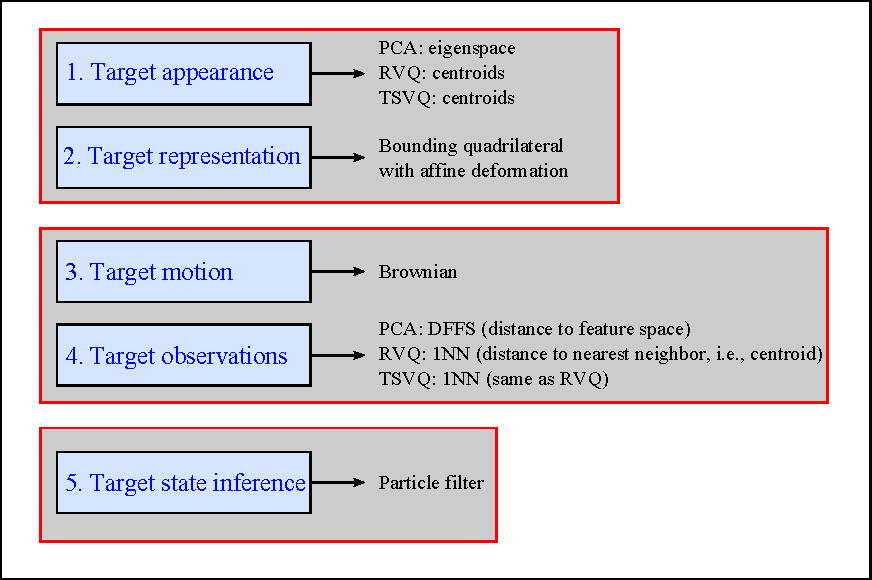
\includegraphics[width=1.0\textwidth]{figs/PhD_experimentalOverview.pdf}
								\caption{Overview.}
								\label{fig:overview}
								\end{figure}

In this chapter, we combine information on target representations presented in Chapter~\ref{chap_Introduction}, theoretical knowledge of RVQ presented in Chaper~\ref{chap_RVQ} and an overview of tracking methods presented in Chapter~\ref{chap_TRK} into a visual tracking framework using RVQ and compare it with visual tracking using PCA and TSVQ.  

This work is significant since PCA is commonly used in the Pattern Recognition, Machine Learning and Computer Vision communities.  On the other hand, TSVQ is commonly used in the Signal Processing and Information Theory communities.  RVQ with more than two stages has not received much attention due to the difficulty in producing stable designs.  In this work, we bring together these different approaches and compare them in a combined visual tracking framework.  The result is a robust tracker for all 3 methods, but with RVQ performing the best according to certain defined criteria to be described later in the chapter.



The approach we take in this work builds on work presented by Ross et. al. in 2008 \cite{2008_JNL_subspaceTRK_Ross}.  As a matter of fact, we have used part of their software with their permission~\cite{2008_SFT_Ross}.  In this spirit, we make our software available for download to the community at \url{https://github.com/SalmanAslamPhD/current}.  

%===================
\section{Background}
%===================
Visual tracking is the task of estimating a target's state over time.  In many cases, the state represents target position and a bounding box around it, or its contour.  However, this is a challenging problem due to the following reasons:

\begin{enumerate}
\item \underline{Appearance and contour changes}:  A target of interest can undergo arbitrary change in appearance and contour.  This can be due to the following reasons:
\begin{enumerate}
\item \underline{Pose change}:  The target can rotate and present a different view to the camera.
\item \underline{Warping}: The target can undergo warps, such as expression changes for humans.
\item \underline{Self occlusion}:  The target can be occluded or unoccluded by itself or its surroundings.
\item \underline{Blur}:  Motion blur can severely distort a target's appearance.
\item \underline{Structured noise}:  The target can change appearance in an orderly manner, for instance, a target of interest can put on or remove glasses or a hat.
\item \underline{Random noise}:  Random noise is added to the light rays coming from a target of interest.  On the hardware side, this is caused by atmospheric effects in the optical channel.  On the receiving side, it is caused by sensor noise, electronics noise and EMI (electromagnetic interference).  On the software side, it can be caused by compression artefacts.
\item \underline{Non-symmetic BRDF}:  The light reflected off of an object in all directions is modeled by the BRDF (Bidirectional Radiation Transfer Function).  Since this function may not be symmetric in all directions, the amount of light reflecting off of the object may be different in different directions.  Multiple cameras viewing the same point will receive different intensity levels.
\end{enumerate}
\item \underline{Lighting change}: Lighting changes can be caused by turning on or off lights in indoor environments, or moving into or out of shades in outdoor environments.
\item \underline{Sudden motion (target or camera)}:  Besides motion blur, sudden motion by the target or camera can cause the target to exit the window in which the tracker looks for the target leading to incorrect track assignment.
\end{enumerate}

								\begin{figure}
								\centering
								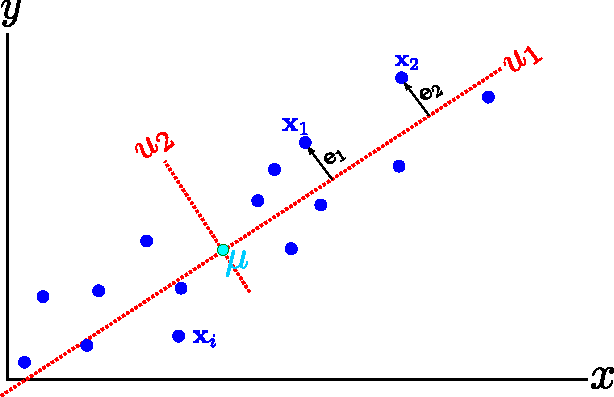
\includegraphics[width=0.45\textwidth]{figs/PRML_PCA_problem.pdf}
								\caption{In $\mathbb{R}^2$, a reduced eigenspace means that eigenvector $u_2$ is discarded.  Vectors $\mathbf{x}_1$ and $\mathbf{x}_2$ have the same projection error on eigenvector $u_1$ even though $\mathbf{x}_1$ is closer to the mean $\boldsymbol\mu$ of the training data $\mathbf{x}_i$.}
								\label{fig:PRML_PCA_problem}
								\end{figure}

For a tracker that tries to learn the appearance and/or contour model of the target, inclusion of background pixels is an added problem that can cause drift.  If none of the problems mentioned above were present, a simple template matching stategy would suffice for robust tracking.  This has complexity $O(nm)$, where $n$ is the number of pixels in the target and $m$ is the number of locations at which the target is searched.  For most practical situations, this does not represent significant computational load and can be done in real time even while tracking several targets.

In this work, we try to address single-target visual-tracking under several of the challenges mentioned above while trying to learn the appearance model of the target.  Seminal work here can be traced back to 1996 when Black and Jepson experimented with tracking using an eigenspace representation of the target appearance model~\cite{1998_JNL_Eigentracking_Black}.  The next notable work is by Moghaddam and Pentland, 1997~\cite{1997_JNL_EigenTRK_Moghaddam} in which they try to address a fundamental limitation of PCA.  In PCA, 2 vectors, $\mathbf{x}_1$ and $\mathbf{x}_2$ can have the same distance to a reduced eigenspace even if they have different distance to the mean of the data.  This is shown for a trivial case in $\mathbb{R}^2$ in Figure~\ref{fig:PRML_PCA_problem} where $\mathbf{e}_1=\mathbf{e}_2=\mathbf{e}$ even though $\mathbf{x}_1$ is closer to the mean $\boldsymbol\mu$ than $\mathbf{x}_2$.  They formulate the problem using DIFS (distance in feature space) and DFFS (distance from feature space) so that both projection error and distance to the mean of the data are used while trying to determine how well the subspace explains a new data-point.  The next breakthrough came with the work of Bishop and Tipping in 1999~\cite{1999_JNL_PPCA_Tipping} where they show that a probabilistic variation of PCA (PPCA) allows PCA to be used as a generative model.  The advantage in tracking is that this methodology allows an assignment of probabilities to new data-points.  This relative weighting can be used to determine best candidates.  All three works were combined into a tracking framework for the first time by Ross et. al. in 2008~\cite{2008_JNL_subspaceTRK_Ross}.  Moreover, they used incremental SVD to make their tracker run in real time.  

								\begin{figure}[t]
								\centering
								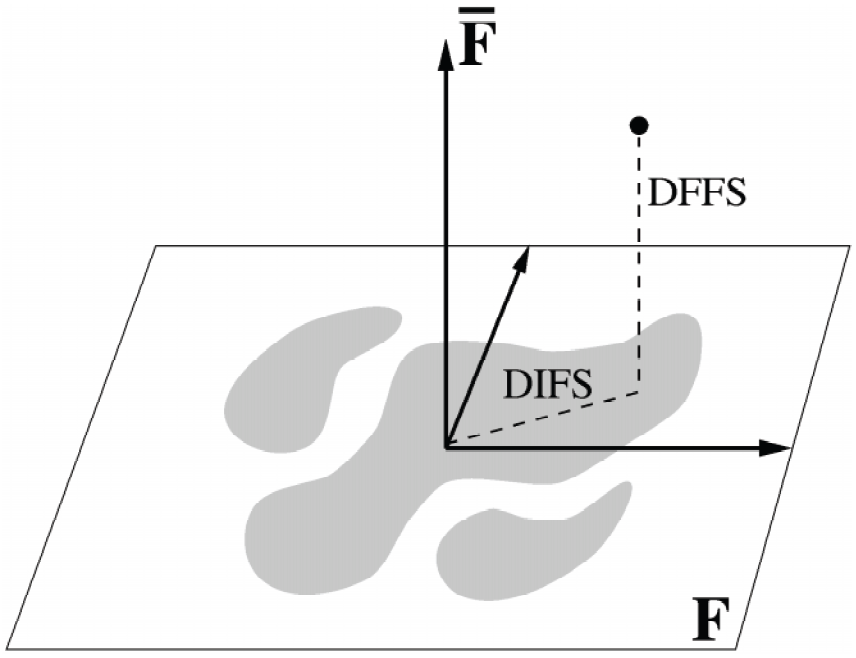
\includegraphics[width=0.5\textwidth]{figs/1998_JNL_ProbVisLearning_Moghaddam_fig3.png}
								\caption{Graphical illustration of DFFS (distance-from-feature-space) and DIFS (distance-in-feature-space).  The feature space is $\mathbf{F}$ while the subspace orthogonal to the feature space is $\bar{\mathbf{F}}$.  DFFS is the signal residual error and DIFS is the $\mathbf{F}$-space likelihood \cite{1997_JNL_EigenTRK_Moghaddam}.}
								\label{fig:1997_JNL_DIFSDFFS_Moghaddam}
								\end{figure}

Here, we extend this work using RVQ instead of PCA and introducing two new distance based measures for relative weighting of tracking candidates.  The result is a generative framework for RVQ that leads to robust tracking.  Whereas RVQ was first introduced by Juang and Gray in 1982~\cite{1982_CNF_SpeechRVQ_JuangGray}, subsequently greatly extended by the seminal work of Barnes~\cite{1991_CNF_DesignPerformanceRVQ_Frost,1992_JNL_RVQ_Barnes,1992_CNF_ImageCodingRVQ_Kossentini,1993_sigmaTrees_Barnes,1993_JNL_RVQDSC_Barnes,1995_JNL_OptimalityRVQ_Kossentini,1996_CNF_VQclassification_Barnes,1996_JNL_AdvancesRVQ_Barnes,2002_JNL_SigmaTrees_Barnes,2004_CNF_DSSAdataMining_Barnes,2007_JNL_Katrina_Barnes,2007_JNL_IDDM_Barnes} and widely known in the signal processing and information theory communities, relatively little attention has been given to this work in the computer vision and machine learning fields where a much simpler version, K-means, has been widely used.  Our goal is to remedy this situation and introduce RVQ in the context of an important and challenging problem, visual target tracking.

%===================
\section{Overview of overall components}
%===================
Our tracking framework is based on five components as shown in Figure~\ref{fig:overview} .  Each of these components is described in detail in later sections.  Here, we present an overview of each:

\begin{enumerate}
\item \underline{ Target appearance}.  Target appearance is modeled using a learned eigenspace, a trained $\sigma$-tree codebook or a binary balanced-tree TSVQ codebook for PCA, RVQ and TSVQ respectively.  Refer to Chapter~\ref{chap_RVQ} for a description of RVQ  $\sigma$-trees.

\item \underline{Target representation}.  Several target representation methods are described in Chapter~\ref{chap_Introduction}.  We use the bounding quadrilateral method.  This quad encloses the pixels of a target of interest.  It is also allowed to warp affinely from frame to frame to minimize inclusion of background pixels as the target changes shape, size and orientation.

\item \underline{Target motion}.  In order to keep our work general, we do not assume any deterministic target motion model.  The target is expected to move according to a Wiener process, i.e., brownian motion.  This allows for robust tracking under arbitrary target and camera motion.

\item \underline{Target observations}.  For PCA, the likelihood of a target observation is assumed proportional to the DFFS (distance to feature space).  DFFS is explained in Chapter~\ref{chap_TRK}.  For RVQ, the likelihood of a target observation is assumed to be proportional to the Euclidean distance to the closest equivalent code-vector.  Equivalent code-vectors are explained in Chapter~\ref{chap_RVQ}.  For TSVQ, the likelihood of a target observation is assumed to be proportional to the Euclidean distance to the closest terminal code-vector.

\item \underline{Target state inference}.  In tracking, the correspondence of observations in the current frame to existing targets in the previous frame is generally an ill-posed problem~\cite{2005_CNF_TRK_Yang}.  We use the particle filter to deal with this problem by propagating multiple hypotheses from frame to frame~\cite{1998_JNL_Condensation_IsardBlake}.

\end{enumerate}

%===================
\section{Overview of temporal process}
%===================
In the previous section, we described the five major components of our visual tracking framework.  In this section, we describe the temporal relationship between these components.  Refer to Figure~\ref{fig:temporal_overview} for a graphical overview.  A brief description of this temporal process is given below while detailed explanation is given in later sections in this chapter.

								\begin{figure}[t]
								\centering
								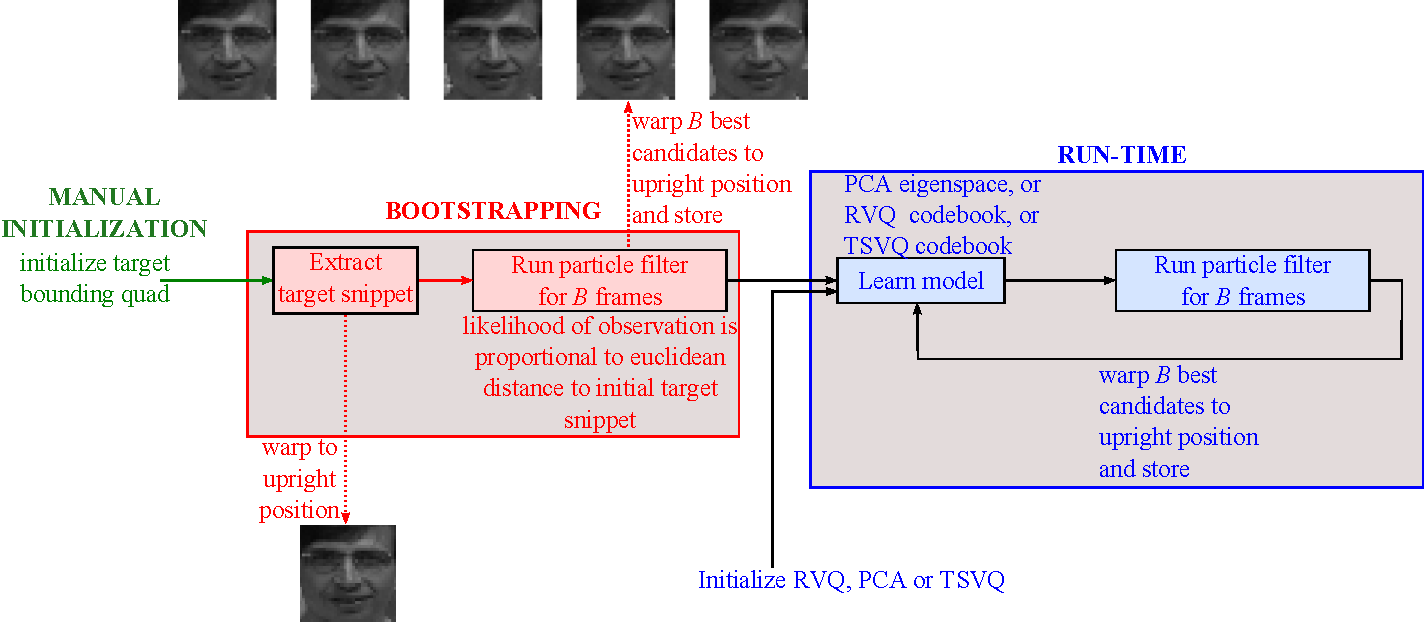
\includegraphics[width=1\textwidth]{figs/PhD_experimentalTemporalOverview.pdf}
								\caption{Temporal overview.}
								\label{fig:temporal_overview}
								\end{figure}


\begin{enumerate}
\item \underline{Manual initialization}.  The target is identified in the first frame by manually drawing a bounding box around it.

%The box is allowed to be affinely deformed as discussed later in this chapter.  Template matching then allows a certain number of frames to be designated as initial training frames.  Currently this value is set to $N_B=5$. 

\item \underline{Bootstrapping}.  A particle filter is run for $B$ frames.  The likelihood of observations is assumed to be proportional to the Euclidean distance from the manually segmented target in the first frame.  The $B$ MAP estimates, i.e. $B$ snippets, one from each of the $B$ frames is stored.

  \item \underline{Run-time}.  During this step, the learning process and the particle run alternately.  For PCA, the learning process includes updating its eigenbasis with the MAP estimates of the particle filter.  For RVQ and TSVQ, the learning process includes updating their codebooks. 
\end{enumerate}


%This model ties in multiple possible spatial observations in a temporal framework to enable sequential inference through the tracking process.
%Every frame after the one-time initialization is tested against the iPCA, bPCA, RVQ and TSVQ models and results are compared.  The Condensation algorithm is used for temporal and spatial integration of observation and state information.  Spatial processing includes generating several candidate window chips (snippets) and picking the one that gives least mean squared reconstruction error.  Temporal processing includes carrying over the posterior density from a frame as the prior density for the next frame.  The snippet that gives the least squared error is retained and added to the pool of training images in FIFO (first-in first-out) fashion, i.e. a moving window of $N_w$ training images is maintained.

The integration of the above-mentioned 5 components in the temporal process just explained enables us to handle the following tracking challenges:

\begin{itemize}

\item Target appearance related
\begin{enumerate}\setcounter{enumi}{0}
\item Target pose changes
\item Lighting changes
\item Structured noise
\item Temporary occlusions
\end{enumerate}

\item Target representation related
\begin{enumerate}\setcounter{enumi}{4}
\item Target scale changes
\item Target orientation changes
\end{enumerate}

\item Target motion related
\begin{enumerate}\setcounter{enumi}{6}
\item Arbitrary camera motion
\item Arbitrary target motion
\end{enumerate}

\end{itemize}


%\begin{itemize}
%\item \underline{Temporary occlusions}.  The occlusions are temporary, on the order of about 10 frames.
%\end{itemize}
%\begin{itemize}
%\item \underline{Perspective changes handled effectively with affine deformation}.  An affine transform in a tracking scenario can deal effectively with a large variety of target deformations, including some perspective effects.  We therefore choose the affine transform in favor of the less restrictive projective transform which can handle severe perspective effects.  A comparison of some 2D geometric transformations is given in Table~\ref{table:2Dtransformations}.
%\end{itemize}

We now discuss each component in our tracking framework (Figure~\ref{fig:overview}).  

%============================
\section{Appearance model}
\label{Sec:RVQ_trk_appearance_model}
%============================
Common appearance models include just the raw values of the pixel intensities~\cite{2000_CNF_TRK_Mallet, 1981_JNL_OpticalFlow_HornSchunck}, pixel intensity distributions~\cite{2002_JNL_MeanShiftFeatureSpaceAnalysis_Comaniciu, 1996_JNL_TRK_Zhu, 2002_JNL_TRK_Paragios, 2002_JNL_TRK_Elgammal}, templates\cite{1997_CNF_TRK_Fieguth}, active appearance models\cite{1998_CNF_ActiveModels_Edwards, 1995_JNL_ActiveModels_Cootes}, pixel intensity centroids~\cite{1997_CNF_TRK_Heisele} and subspace based methods~\cite{1997_JNL_EigenTRK_Moghaddam, 1998_JNL_Eigentracking_Black}.  

In this work, we use RVQ pixel intensity centroids for the appearance model in RVQ based visual tracking.  We compare RVQ tracking with pixel intensity centroids 

Several appearance models have been The appearance model of a target could 
In this work, we use 3 different learning algorithms.  Each of these algorithms uses its own appearance model.  We discuss these one by one.

%----------------------------
\subsection{RVQ}
%----------------------------
The appearance model in this work depends on which le
The appearance model of a target is an abstraction for the intensity values of its pixels.  

In this work, we choose three appearance models based on PCA, RVQ and TSVQ.  In each case, the appearance model is updated every $N_B$ frames, chosen to be 5 in this work for accurate comparison with~\cite{2008_JNL_subspaceTRK_Ross}.    This updating allows the tracker to deal with changing target pose, lighting changes, structured noise and temporary occlusions.   




\newpage
At every frame, we try to estimate a state vector $\mathbf{X}$ in $R^6$.  Two components of this vector, the target coordinates are related to the motion model and the remaining four are related to the affine deformation allowed by the representation model.  To keep our models as general as possible, all 6 components of the state are modeled as Gaussian random variables but with known variance.  However, in order to simplify sampling from the joint density, it is possible to use certain relaxation criteria such as Markovian dependence, or complete independence.  We choose the latter to make the sampling process in the inference model somewhat more straightforward.

Our motion model then consists of 6 uncorrelated gaussian densities. 
The target motion is therefore represented not in analytic form but as a 6x6 diagonal covariance matrix $\Sigma_X$ centered at the target position $\mathbf{X}_{t-1}$ in the previous frame.  The elements on the diagonal represent variances of affine parameters, $\sigma_x^2, \sigma_y^2, \sigma_\theta^2, \sigma_s^2, \sigma_\alpha^2, \sigma_\phi^2$.   


Several Gaussian distributions are used to handle these changes.  One distribution each is used to handle arbitrary translation in the horizontal direction, vertical direction, scale, rotation.  At every time step, predicted values are sampled from these distributions.  Each predicted value is warped to a standard window size and tested against the existing model.  The predicted value closest to the current model is selected as the next estimate and is used to update the model.  In PCA, the model is the eigenvectors, in RVQ, it's the stage codevectors and in TSVQ, it's the terminal codevectors.  

In this work, we model the object motion by an affine image warp.  The state at time $t$ consists of 6 affine transformation parameters: $x_t,  y_t, \theta_t, s_t, \alpha_t$, and $\phi_t$.



We now look at each of these methods in turn.

%----------------------------------------------
\subsection{PCA}
%----------------------------------------------

In this work, for PCA, it is assumed that an image $\mathbf{X}$ in $R^D$ is probabilistically generated from a subspace $\mathbf{U}$ spanned by earlier observed images.  The covariance matrix $\Sigma$ of the input training images can be written as follows,  

\begin{equation}
\Sigma = \mathbf{U}\mathbf{\Lambda} \mathbf{V}^T
\end{equation}

Here $\mathbf{\Lambda}$ is the matrix of eigenvalues.  The distribution is assumed to be Gaussian centered at $\mathbf{\mu}$.  The probability of an image being generated under this distribution is inversely proportional to its distance from $\mathbf{\mu}$.  This distance can be decomposed into two parts:

\begin{enumerate}
\item DFFS (distance-from-feature-space):  In a partial KL expansion using $Q$ eigenvectors, the space spanned by these $Q$ eigenvectors is given by $\mathbf{F}$ and the signal residual $\epsilon^2$ is given by

\begin{equation}
\epsilon^2 = \Vert \tilde{\mathbf{X}} \Vert^2 - \sum\limits_{i=1}^M \mathbf{u}_i^2 = \sum\limits_{i=M+1}^D \mathbf{u}_i^2
\end{equation}

where $\mathbf{u}_i$ are the eigenvectors of $\Sigma\Sigma^T$ and $\tilde{\mathbf{X}}$ is the mean removed input image.  This signal residual is referred to as DFFS.
\item DIFS (distance-in-feature-space):  This is the component of $\mathbf{X}$ which lies in the feature space $\mathbf{F}$.  
\end{enumerate}

DIFS and DFFS are illustrated graphically in Figure~\ref{fig:1997_JNL_DIFSDFFS_Moghaddam}.  

%This leads the likelihood function to be a function of two distributions,
%
%\begin{equation}
%p(\mathbf{I}|\mathbf{X}) =  \mathcal{N}()
%\end{equation}
%
%\begin{equation}
%p(I_t|X_t) = \mathcal{N}
%\end{equation}

%----------------------------------------------
\subsection{RVQ}
%----------------------------------------------
For RVQ, the appearance model is exactly the same as that used in Chapter~\ref{chap_RVQ_CV_recog}.  The only difference is that the codebooks are now dynamic and updated every $N_B=5$ frames. 

%----------------------------------------------
\subsection{TSVQ}
%----------------------------------------------

The Tree Structured Vector Quantizer (TSVQ) has received a lot of attention in the literature~\cite{1991_BOOK_VQ_GershoGray}.  The reason is that the codebook produced by a TSVQ approximates the codebook produced by an Exhaustive Search Vector (ESVQ) but the run-time computational cost is logarithmic in the number of code-vectors.  The storage requirements however are greater.  A comparison of ESVQ, TSVQ and RVQ can be seen in Table~\ref{tab:comparison_ESVQ_TSVQ_RVQ}.

In TSVQ design, the first step is to compute the mean of the data.  All the data is mapped to this mean.  The mean is then split off into $M_{TSVQ}$ centroids (code-vectors).  For a binary TSVQ, $M=2$.  The data is mapped to these centroids using the Nearest Neighbor rule.  Each of these $M_{TSVQ}$ parent centroids is then again split into $M_{TSVQ}$ child centroids.  Splitting can be achieved by multiple iterations of the K-means algorithm to get centroids that give low mean squared error.  At every stage of the tree, data belonging to a parent code-vector is mapped to the child code-vectors after the splitting occurs.  Notice that the important code-vectors are the last stage children code-vectors, i.e. the terminal leaves of the tree.  However, during run-time, the parent code-vectors, i.e., the non-terminal nodes of the tree have to be stored in order to be able to traverse the tree to get to the terminal code-vectors.  The process of mapping data at run-time to the terminal code-vectors is quite straightforward.  The data is first mapped to the mean, which is a trivial step, since all data starts at the top of the tree, i.e., the mean.  Each data-point is then mapped to one of the two children nodes at the first stage using the Nearest Neighbor method.  This process continues till a terminal code-vector is reached which is then used as an approximation to the input data-point.

In this work, we use a binary and balanced TSVQ.  In the binary case, the storage requirements are double the storage requirements for an equivalent ESVQ.  However, the run-time savings decrease logarithmically.  For instance, a codebook size of $K=256$ requires 256 matches for ESVQ but only 8 matches for a binary TSVQ.  

During tracking, a TSVQ codebook is designed every $N_B=5$ frames using $N_w$ images in the training buffer.  The particle filter candidate target regions in the current frame are tested against this code-book, i.e., for each candidate region, the terminal code-vector  to the mean squared error between that region and the terminal code-vector in the tree that 

The candidate that gives least mean squared error is chosen as the most likely  to find the terminal code-vector in the TSVQ tree that minimizes mean-squared error.  


%=======================		
\section{Representation model}
\label{Sec:Representation_model}
%=======================		
In this section, we discuss the representation model.  We refer back to Figure~\ref{fig:TRK_objectRepresentations} in the introductory chapter that shows different target representations.  




								\begin{figure}[t]
								\centering
								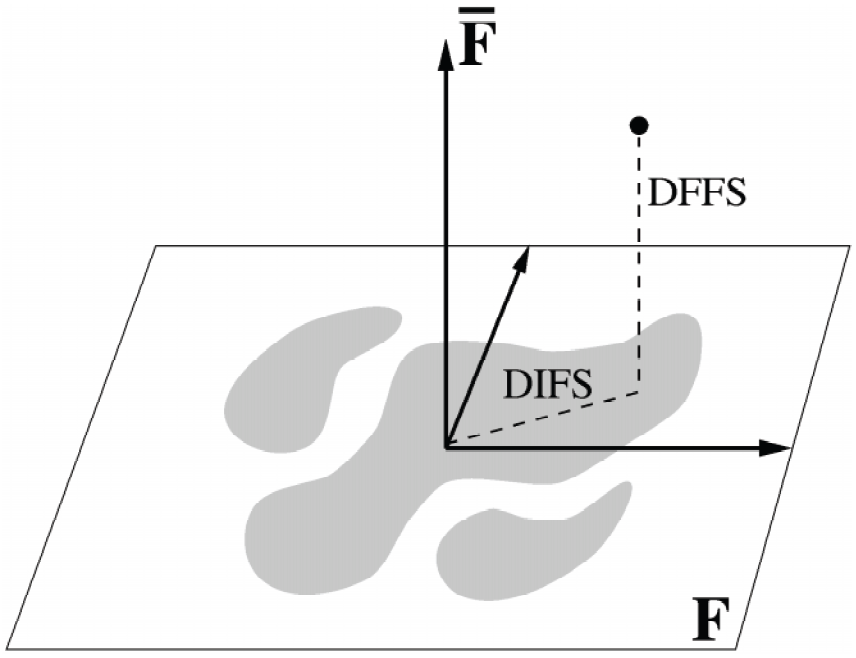
\includegraphics[width=0.5\textwidth]{figs/1998_JNL_ProbVisLearning_Moghaddam_fig3.png}
								\caption{Graphical illustration of DFFS (distance-from-feature-space) and DIFS (distance-in-feature-space).  The feature space is $\mathbf{F}$ while the subspace orthogonal to the feature space is $\bar{\mathbf{F}}$.  DFFS is the signal residual error and DIFS is the $\mathbf{F}$-space likelihood \cite{1997_JNL_EigenTRK_Moghaddam}.}
								\label{fig:1997_JNL_DIFSDFFS_Moghaddam}
								\end{figure}





%=======================		
\section{Motion model}
%=======================		
The motion model is a mathematical representation of the real or expected motion of the target of interest.  Since tracking is in general an ill-posed problem, it is common to make assumptions about the motion to simplify motion modeling.  Common assumptions such as stationary camera, coherent motion etc. are discussed in Chapter~\ref{chap_Tracking_methods}.

In this work, we make two assumptions about the target motion:

\begin{itemize}
\item \underline{Coherent motion}.  We assume that each part of the target moves together.  The target can deform and warp but it does not break up into individual parts.
\item \underline{Can be modeled with a gaussian distribution with fixed variance}.  We assume that the motion is brownian and can be modeled with a gaussian distrubution with a fixed variance.  
\end{itemize}

An advantage of not having an explicit motion model is that arbitrary camera and target motion are allowed.  A disadvantage of this approach in the context of the particle filter is that particles need to be evaluated all around the current target position, rather than only around the projected target position.  We are therefore unable to take advantage of the reduced spatial search-space that comes with a deterministic motion model.  

Two of the six components of the state vector $\mathbf{X}$ deal with the motion model.  These are the $x$ and $y$ coordinates of the target.  These are modeled as independent gaussian random variables with fixed variance $\sigma_x^2, \sigma_y^2$,

\begin{align*}
p(x_t|x_{t-1}) &= \mathcal{N}(x_{t-1}, \sigma_x^2) \\
p(y_t|y_{t-1}) &= \mathcal{N}(y_{t-1}, \sigma_y^2) \\
\end{align*}

%=======================		
\section{Observation model}
%=======================		
An observation model $p(z_t|x_t)$ relates the state $x_t$ at time $t$ to the observation $z_t$ at time $t$.  Unfortunately, it is not possible to estimate it from the data and so reasonable assumptions must be made.  The observations are assumed to be independent of each other as well as of the dynamical process \cite{1998_JNL_Condensation_IsardBlake}. 

In this work, for PCA, the observation model assumes that the candidate window chips (snippets) in the image that can contain the target were generated from a subspace of the target $\mathbf{U}$ centered at $\mathbf{\mu}$.  The distance metric used to score each candidate window is explained in Section~\ref{Sec:Chap5_PCA}.  For RVQ and TSVQ, the observation model assumes that the candidate snippets were generated from the RVQ and TSVQ codebooks respectively.  The distance metric used to score snippets is based on the mean squared reconstruction error.  For RVQ, an additional constraint is monotonic SNR increase in the DSSA (direct sum successive approximation) reconstruction.  In other words, not all RVQ stages have to be used to reconstruct the target.  The reconstruction must stop if the stage code-vector at the next additive stage does not result in SNR increase.


It has been shown by Roweis and Ghahramani~\cite{1999_JNL_Gaussian_roweis} that under the assumption of gaussian noise, factor analysis (FA), principal component analysis (PCA), mixtures of gaussian (MoG) clusters, vector quantization (VQ), independent components analysis (ICA), Kalman filters and hidden Markov models (HMMs) are instances of a single basic generative model, the linear gaussian model.  The linear gaussian model can be written as,

\begin{equation}
\begin{array}{llllllllllllll}
\mathbf{x}_{t+1} &=  \mathbf{A}\mathbf{x}_{t} +  \mathbf{w}_t   & & & \mathbf{w}_t \sim \mathcal{N}(0, \mathbf{Q})\\
\mathbf{y}_t 		 &=  \mathbf{C}\mathbf{x}_{t} +  \mathbf{v}_t    & & & \mathbf{v}_t \sim \mathcal{N}(0, \mathbf{R})
\end{array}
\label{LGM}
\end{equation}

where $\mathbf{A}$ is the state transition matrix, $\mathbf{C}$ is the observation matrix, and $\mathbf{w}_t$ and $\mathbf{v}_t$ are zero-mean gaussian random variables.  Under conditions where each data point $\mathbf{x}$ was generated independently and identically without any temporal ordering, i.e., $\mathbf{A}=\mathbf{0}$, we can write,

\begin{equation}
\begin{array}{llllllllllllll}
\mathbf{x} &= \mathbf{w} 											& & & \mathbf{w} &\sim \mathcal{N}(0, \mathbf{Q})\\
\mathbf{y} &=  \mathbf{C}\mathbf{x} +  \mathbf{v} 		& & & \mathbf{v} & \sim \mathcal{N}(0, \mathbf{R})
\end{array}
\label{LGM1}
\end{equation}



\begin{table}[t]
\centering
\begin{tabular}{| c | c | c | c | c |}\hline
 				 	&\textbf{A}	 	&	\textbf{C}  									& \textbf{Q} 	&  \textbf{R}                                                                		\\\hline
\textbf{PCA} 	&\textbf{0}		&	principal eigenvectors of $\boldsymbol\Sigma$	& \textbf{I}  	&  $\lim\limits_{\sigma^2 \rightarrow 0} \sigma^2\mathbf{I}$ 	\\\hline
\textbf{PPCA} &\textbf{0}		& 	scaled principal eigenvectors of $\boldsymbol\Sigma$	& \textbf{I}	&										      $\sigma^2 \mathbf{I}$	 \\\hline
\textbf{FA}   	&\textbf{0}		&													& \textbf{I} 	&  diagonal matrix 																\\\hline
\textbf{VQ}	 	&\textbf{0} 	&	cluster means								& \textbf{I}	& 	-																					\\\hline
\end{tabular}
\caption{Unifying PCA, PPCA, FA, and VQ using linear gaussian models~\cite{1999_JNL_Gaussian_roweis, 1999_JNL_PPCA_Tipping}.}
\label{table:LGM_unifying}
\end{table}

Moreover, for non-linear mappings, such as in MoG and VQ, a function $\mathbf{WTA[.]}$, \emph{winner-take-all} is introduced which returns a vector with unity in one position and all remaining zeros,

\begin{equation}
\begin{array}{llllllllllllll}
\mathbf{x} &= \mathbf{WTA}(\mathbf{w}) 						& & & \mathbf{w} &\sim \mathcal{N}(\mathbf{\boldsymbol\mu}, \mathbf{Q})\\
\mathbf{y} &=  \mathbf{C}\mathbf{x} +  \mathbf{v} 		& & & \mathbf{v} & \sim \mathcal{N}(0, \mathbf{R})
\end{array}
\label{LGM2}
\end{equation}

The values for \textbf{A}, \textbf{C}, \textbf{Q} and \textbf{R} under this elegant, unifying generative framework for various algorithms, including PCA and VQ, are given in Table~\ref{table:LGM_unifying}.  Besides being inherently satisfying, this framework allows the computation of data likelihoods in the case of PCA and VQ since they both do not define a proper density in the observation space~\cite{1999_JNL_Gaussian_roweis}.  We start with likelihoods under PCA, PPCA and VQ.  Our contribution is extending this work to compute likelihoods under RVQ.

\subsection{Likelihood for PCA}
%-----------------------------------------
In a gaussian distribution, the probability of a data point $\mathbf{x}$ in $\mathbb{R}^D$ depends on the Mahalanobis distance $d$.  The output of PCA, zero-centered $\mathbf{\tilde{y}}$ is decorrelated with variances along each dimension equal to the eigenvalues $\lambda_i$ of the covariance matrix $\boldsymbol\Sigma$,


\begin{equation}
\begin{array}{lllllll}
d &= (\mathbf{x}-\boldsymbol\mu)^T\boldsymbol\Sigma^{-1}(\mathbf{x}-\boldsymbol\mu)\\
&=\mathbf{\tilde{x}}^T\boldsymbol\Sigma^{-1}\mathbf{\tilde{x}}\\
&=\mathbf{\tilde{x}}^T(\mathbf{U}\boldsymbol\Lambda\mathbf{U}^T)^{-1}\mathbf{\tilde{x}}\\
&=\mathbf{\tilde{x}}^T(\mathbf{U}\boldsymbol\Lambda^{-1}\mathbf{U}^{-1})\mathbf{\tilde{x}}\\
&=(\mathbf{U}^T\mathbf{\tilde{x}})^T\boldsymbol\Lambda^{-1}(\mathbf{U}^T\mathbf{\tilde{x}})	\\
&=\mathbf{\tilde{y}}^T\boldsymbol\Lambda^{-1}\mathbf{\tilde{y}}\\
&=\sum\limits_{d=1}^D \frac{\tilde{y}_i}{\lambda_i}\\
&=\sum\limits_{d=1}^Q \frac{\tilde{y}_i^2}{\lambda_i} + {\color{red}\sum\limits_{d=Q+1}^D} \frac{{\color{red}\tilde{y}_i^2}}{\lambda_i}, \ \ \  & \bigg(\textrm{DFFS = recon. error}={\color{red}\sum\limits_{i=1}^D e_i^2} = \sum\limits_{i=1}^D \tilde{x}_i^2 - \sum\limits_{i=1}^Q \tilde{y}_i^2= {\color{red}\sum\limits_{d=Q+1}^D} {\color{red}\tilde{y}_i^2}\bigg)\\
&=\sum\limits_{d=1}^Q \frac{\tilde{y}_i^2}{\lambda_i} + \frac{1}{\rho} {\color{red}\sum\limits_{i=1}^D e_i^2} \ \ \ & \bigg(\rho^* = \frac{1}{D-q}\sum\limits_{i=q+1}^D \lambda_i\bigg)\\
\end{array}
\label{Eqn:MoghaddamLikelihood}
\end{equation}

This formulation, first presented in~\cite{1997_JNL_EigenTRK_Moghaddam} shows that the first term in the sum is the DIFS term in Figure~\ref{fig:1997_JNL_DIFSDFFS_Moghaddam} while the second term corresponds to DFFS.  With this formulation, PCA can be used in a probabilistic framework since the error of a test vector $\mathbf{x}$ now also depends on its distance from the mean of the data.

\subsection{Likelihood for PPCA}
%-----------------------------------------
For PCA, using Equation~\ref{LGM1} and Table~\ref{table:LGM_unifying}, we have the likelihood of observing $\mathbf{y}$ given by,

\begin{equation}
p(\mathbf{y}) \sim \mathcal{N}(\boldsymbol\mu, \mathbf{C}\mathbf{C}^T + \sigma^2 \mathbf{I})
\end{equation}

Bishop and Tipping~\cite{1999_JNL_PPCA_Tipping} show that this can be done in closed form using PPCA with the following solution,

\begin{equation}
\begin{array}{lllll}
\mathbf{\boldsymbol\mu}_{\textrm{ML}} &=\frac{1}{N}\sum\limits_{i=1}^N \mathbf{x}_i\\
\sigma^2_{\textrm{ML}} &= \frac{1}{D-q}\sum\limits_{i=q+1}^D \lambda_i\\
\mathbf{C}_{\textrm{ML}} &= \mathbf{U}_q(\mathbf{\Lambda}_q - \sigma^2\mathbf{I})^{1/2} \\
\end{array}
\label{Eqn:PPCA}
\end{equation}

where, $\boldsymbol\Sigma = \mathbf{U}\mathbf{\Lambda}\mathbf{V}^T$, $\mathbf{U}_q$ are the first $q$ eigenvectors in $\mathbf{U}$, $\mathbf{\Lambda}_q$ contains the corresponding eigenvalues, $\lambda_1, \lambda_2, \ldots \lambda_q$, $D$ is the dimensionality of the data and $N$ is the number of data points.  Note that in the above equation, we have omitted multiplication with an arbitrary rotation matrix since it can be taken to be $\mathbf{I}$ without loss of generality.  

In Equation~\ref{Eqn:PPCA}, $\sigma^2_{\textrm{ML}}$ is the average variance in the discarded dimensions and $\mathbf{C}_{\textrm{ML}}$ maps $\mathbf{x}$ onto its principal components to give output $\mathbf{y}$.





\subsection{Likelihood for VQ}
%---------------------------------
As mentioned earlier, VQ does not define a proper density in the observation space.  Moreover, in the linear gaussian model, Table~\ref{table:LGM_unifying} shows that in VQ, similar to PCA, the observation noise vanishes, $\lim\limits_{\sigma^2 \rightarrow 0} \sigma^2\mathbf{I}$.  The posterior therefore collapses to a single point, and all its mass is centered on the nearest centroid.  In this case, the likelihood of a data point $\mathbf{x}_i$ is proportional to its squared distance from the nearest centroid.

\subsection{Likelihood for RVQ}
%---------------------------------
In this work, we introduce a new distance measure $d_r$ for RVQ.  Its role is similar to the role played by the Mahalanobis distance in probabilistic PCA.  Essentially, it is used to assign a probability measure to a new data point and demonstrates how well this data point is explained by the RVQ codebook $\Phi$.  The RVQ codebook $\Phi$ is generated using training data and 3 parameters, target decoding SNR, $S$, maximum number of stages, $Q_{\textrm{max}}$ and number of codevectors per stages, $M$.  $d_r$ is given by,




\begin{equation}
d_r = \dr
\end{equation}

Here, $\boldsymbol\mu_k$ is closest centroid to $\mathbf{x}_i$, $Q_i$ is the number of stages required to decode $\mathbf{x}_i$, and $\lambda$ is a regularization parameter.  With this distance measure, the likelihood of a data point being generated by an RVQ codebook $\Phi$ is given by,

\begin{equation}
p(\mathbf{x}_i|\Phi) = \frac{e^{-\big(\dr\big)}} {\sum\limits_{i=1}^N e^{-\big(\dr\big)}}
\end{equation}

\begin{enumerate}
\item \underline{maxQ}: In this method, RVQ decoding is carried out so that maximum stages $Q$ are used.
\item \underline{RofE}: In this method, realm of experience coding is used.  A test vector is decoded such that the decode path traversed belongs to the set of training decode paths.
\item \underline{nulE}: In this method, null encoding is used.  Reconstruction rms error is checked at every stage.  If at any stage, rms error is not reduced, that stage is skipped until maximum stages are attained.
\item \underline{monR}: In this method, monotonic rms error is a condition.  If this condition is not met, decoding stops.
\end{enumerate}


%=======================		
\section{Inference model}
%=======================		
The inference model in this work is based on a sequential Monte Carlo (SMC) filter, the particle filter.  The particle filter has been discussed in Chapter~\ref{chap_Tracking_methods}.  Almost all particle filters are based on the sequential importance sampling (SIS) algorithm, including the sampling importance resampling (SIR) filter, auxiliary sampling importance resampling (ASIR) filter and the regularized particle filter (RPF).  The basic difference between these algorithms is the choice of \emph{importance sampling density} and/or modification of the resampling step~\cite{2002_JNL_PF_Arulampalam}.  

In this work, we use the basic SIS algorithm.  It is essentially the same as the SIR filter except that there is no resampling step.  However, like the SIR filter, we use the prior density as the importance sampling density.  The weights on the posterior are computed using the appearance model for PCA, RVQ or TSVQ, depending on which of these algorithms is being used.  For RVQ for instance, the mean squared reconstruction error is used for the weighting.

The number of particles used is $N_p=600$.  Each particle represents the point mass density of a vector $\mathbf{X}$ in $R^6$ corresponding to the 6 parameters required for an affine deformation.

\cite{1992_JNL_MCMC_Carlin}








%===========================
\section{Results}
%===========================
\begin{table}[t]
\footnotesize
\begin{tabular}{p{0.6in}|p{0.6in}p{0.6in}p{0.4in}p{0.4in}cccccc}
Dataset 		&Scenario	     &\parbox[c]{0.4in}{\center Time of \\day} 	&\parbox[c]{0.26in}{\center Target of \\interest}  &\parbox{0.3in}{\center Rigid \\target} 	&\parbox{0.4in}{\center Lighting change 1-5 \\(5 most severe)}  	&\parbox{0.5in}{\center Structured \\noise} 	&\parbox{0.4in}{\center Camera \\motion} 	&\parbox{0.3in}{\center Pose \\change} 	&\parbox{0.45in}{\center Expression \\change} 	&\parbox{0.3in}{\center Temporary \\occlusion} 	\\\hline
Dudek 			&Indoors 	     &N/A 			&human 					&no 	&1 	&yes 	&yes 	&yes 	&yes 	&yes 		\\\hline
davidin300 	&Indoors		&N/A			&human					&no	&2	&yes	&yes	&yes	&yes	&no		\\\hline
sylv				&Indoors		&N/A			&toy						&yes	&4	&no	&yes	&yes	&N/A	&no		\\\hline
trellis70	 		&Outdoors 		&day, dark		&human					&no	&5	&no	&yes	&yes	&yes	&no		\\\hline
fish				&Indoors		&N/A			&object					&yes	&4	&no	&yes	&no	&N/A	&no		\\\hline
car4			&Outdoors 		&day, sunny	&vehicle					&yes	&3	&no	&yes	&yes	&N/A	&no		\\\hline
car11			&Outdoors		&night			&vehicle					&yes	&4	&no	&yes	&yes	&N/A	&no		\\\hline
\end{tabular}
\caption{Datasets used for RVQ tracking.}
\label{Tab:datasets_used}
\end{table}


\begin{table}[h!]
\centering
\begin{tabular}{|l|c|c|c|}
\hline
&\textbf{PCA}&\textbf{TSVQ}&\textbf{RVQ}\\\hline
\textbf{Dudek}&7.44&8.62&6.68\\\hline
\textbf{davidin300}&4.60&5.93&4.29\\\hline
\textbf{sylv}&4.34&4.61&4.19\\\hline
\textbf{fish}&2.17&4.59&2.60\\\hline
\textbf{car4}&4.60&5.11&4.72\\\hline
\textbf{car11}&2.13&2.21&2.00\\\hline
\textbf{mean}&4.21&5.18&4.08\\\hline
\end{tabular}

\caption{Comparison of best possible tracking error between PCA, RVQ and TSVQ over all algorithm parameters for 6 publicly available challenging datasets, Dudek, davidin300, sylv, fish, car4 and car11.  The table shows that RVQ produces the best results for 4 of the 6 datasets.  Overall tracking error is least for RVQ followed by PCA, and then followed by TSVQ.}
\end{table}

\begin{table}[h!]
\centering
\input{tables/tables_comparison_DOF_16}
\caption{Comparison of tracking results using the same DoF, 16 eigenvectors for PCA, 8x2 RVQ and 3x2 TSVQ (15 DOF for TSVQ, 8 terminal code-vectors and 7 stage code-vectors).  RVQ has best overall tracking performance.}
\end{table}

\begin{table}[h!]
\centering
\input{tables/tables_comparison_DOF_32.tex}
\caption{Comparison of tracking results using the same DoF, 32 eigenvectors for PCA, 8x4 RVQ and 4x2 TSVQ (31 DOF for TSVQ, 16 terminal code-vectors and 15 stage code-vectors).  RVQ has best tracking performance every time, and therefore also best overall performance.}
\end{table}


For the interested reader, the appendix contains detailed results for tracking errors for all 6 datasets, for all RVQ types (maxQ, RofE, nulE, monR), over several RVQ configurations (8x2, 8x4, 8x8, 8x12, 8x16).  Also, detailed graphical results for all 6 datasets, for all RVQ types, for the 8x4 configuration are also presented.











